\chapter{背景}

\section{概述}
概率图模型(Probabilistic Graphical Model, PGM),简称图模型(Graphical Model,GM),是指一种用图结构来描述多元随机变量之间条件独立性的概率模型(注意条件独立性),从而给研究高维空间的概率模型带来了很大的便捷性。

对于一个$K$维的随机向量,其联合概率为高维空间中的分布,一般难以直接建模。假设每
$\mathbf{X}=[X_1,X_2,\cdots,X_K]^T$个变量为离散变量并且有$m$个取值,在不做任何独立假设条件下
,则需要$m^K-1$个参数才能表示其概率分布。

参数数量是指数级的,这在实际应用中不可接受,而一种可以有效减少参数量的方法就是\textsl{独立性假设}。将
$K$维随机向量的联合概率分解为$K$个条件概率的乘积
\begin{equation}
    \begin{aligned}
         p(\mathbf{x}) &=P(\mathbf{X}=\mathbf{x})\\
         & = p(x_1)p(x_1|x_2)\cdots p(x_k|x_1,x_2,\cdots,x_{K-1})\\
         & = \prod\limits_{k=1}^{K}p(x_k|x_1,\cdots,x_{k-1})
    \end{aligned}
\end{equation}

如果某些变量之间存在条件独立,则其参数量可以大幅度减少。假设有四个二值变量,在不知道这几个变量依赖关系的情况下,用一个联合概率表来记录每一种取值的概率需要
$2^4-1=15$个参数,则在已知$\mathbf{X}_1$时,$\mathbf{X}_2$和$\mathbf{X}_3$独立,即有
\begin{equation}
    p(x_2|x_1,x_3)=p(x_2|x_1)
\end{equation}

同理:$p(x_3|x_1,x_2)=p(x_3|x_1)$

因此假如我们知道更多独立性条件,可以大大简化联合概率分布的计算,而\textsl{概率图}则可以直观表示
随机变量之间条件独立性关系。

\subsection*{概率图模型的三个基本问题}

\begin{enumerate}
    \item 表示问题:对于一个概率模型,如何通过图结构描述变量之间的依赖关系;
    \item 学习问题:图模型的学习包括图结构的学习和参数的学习,即参数估计问题;
    \item 推断问题:计算其他变量的条件概率分布;
\end{enumerate}

\subsection*{有向图模型}

有向图模型(Directed Graphical Model),也称为贝叶斯网络(Bayesian Network)或信念网络(Belief Network,BN),是一类用有向图来描述随机向量概率分布的模型。常见的有向图模型:很多经典的机器学习模型可以使用有向图模型来描述,比如朴素贝叶斯分类器、隐马尔可夫模型、深度信念网络等。

\subsection*{无向图模型}

无向图模型,也称为马尔可夫随机场(Markov Random Field,MRF)或马尔可夫网络(Markov Network),是一类用无向图来描述一组具有局部马尔可夫性质的随机向量 $\mathbf{X}$
 的联合概率分布的模型。常见的无向图模型有:最大熵模型、条件随机场、玻尔兹曼机、受限玻尔兹曼机等。

\section{极大似然估计(maximum likelihood estimation)}

给定概率分布$D$,已知其概率密度函数(连续分布)或者概率质量函数(离散分布)为$f_D$,
以及一个分布参数$\theta$,我们可以从这个分布中抽一个具有$n$个值的采样$X_1,X_2,\cdots,X_n$,利用
$f_D$计算出其似然函数
\begin{equation}
    L(\theta|x_1,\cdots,x_n)=f_\theta(x_1,\cdots,x_n)
\end{equation}

若$D$是离散分布,$f_\theta$即是在参数为$\theta$时观测到这一采样的概率;
若其是连续分布,$f_\theta$则为$X_1,X_2,\cdots,X_n$联合分布的概率密度函数
在观测值处的取值。

从数学上来说,我们可以在$\displaystyle \theta$的所有可能取值中寻找一个值使得似然函数取到最大值。这个使可能性最大的
$\displaystyle {\widehat {\theta }}$值即称为$\displaystyle \theta$的最大似然估计。由定义,最大似然估计是样本的函数。

\subsection*{相对熵}

最大似然估计可以从相对熵推导而来。相对熵衡量了使用一个给定分布$Q$来近似另一个分布
$P$时的信息损失,对于离散随机变量
\begin{equation}
    D_{KL}(P||Q)=\sum_{i}P(i)log\frac{P(i)}{Q(i)}
\end{equation}

其中$P$是真实分布,$Q$是近似分布。在最大似然估计的情景下,假设分布拥有一系列参数$\theta$,
我们希望通过样本得到参数的估计值$\hat{\theta}$,我们可以利用相对熵来评估估计的好坏
\begin{equation}
    D_{KL}(p_\theta(x)||p_{\hat{\theta}}(x))=\sum_{x\in E}p_\theta(x)log \frac{p_\theta(x)}{p_{\hat{\theta}}(x)}
\end{equation}

根据数学期望的定义,上式可以改写
\begin{equation}
    D_{KL}(p_\theta(x)||p_{\hat{\theta}}(x))=\mathbb{E}_\theta[log(\frac{p_\theta(x)}{p_{\hat{\theta}}(x)})]
    =\mathbb{E}_\theta[log\ p_\theta(x)]-\mathbb{E}_\theta[log\ p_{\hat{\theta}}(x)]
\end{equation}

KL值越大,参数估计越坏,因此,需要通过改变估计参数$\hat{\theta}$的值来获得最小的值,所对应的参数极为最佳估计参数
\begin{equation}
    \hat{\theta}_{best}=arg\ \min\limits_{\hat{\theta}}\ D_{KL}(p_\theta(x)||p_{\hat{\theta}}(x))
\end{equation}

假设有$n$个样本,根据\textsl{大数定律},
\begin{equation}
    \mathbb{E}_{\theta}[log\ p_{\hat{\theta}(x)}]\rightsquigarrow \frac{1}{n}\sum\limits_{i=1}^{n}log\ p_{\hat{\theta}}(x)
\end{equation}

因此我们可以通过下式去估计
\begin{equation}
    D_{KL}(p_{\theta}(x)||p_{\hat{\theta}}(x))=\mathbb{E}_{\theta}[log\ p_{\theta}(x)]-\frac{1}{n}\sum\limits_{i=1}^{n}log\ p_{\hat{\theta}}(x_i)
\end{equation}

对于一个已知的分布,其参数$\theta$是确定的。因此,$\mathbb{E}_{\theta}[log\ p_{\hat{\theta}(x)}]$为常数。因此,我们可以通过最小化KL值获得最佳估计参数:

\begin{equation}
    \hat{\theta}=arg\ \min\limits_{\theta}\ \mathbb{E}_{\theta}[log\ p_{\hat{\theta}(x)}]-\frac{1}{n}\sum\limits_{i=1}^{n}log\ p_{\hat{\theta}}(x_i)
\end{equation}

只要求和项最大,那么整体就最小,这个优化问题等价于
\begin{equation}
    \begin{aligned}
        & arg\ \max\limits_{\theta}\ \frac{1}{n}\sum\limits_{i=1}^{n}log\ p_{\hat{\theta}}(x_i)\\
        & \Rightarrow arg\ \max\limits_{\theta}\ log[\prod\limits_{i=1}^{n}p_{\hat{\theta}}(x_i)]\\
        & \Rightarrow arg\ \max\limits_{\theta}\ \prod\limits_{i=1}^{n}p_{\hat{\theta}}(x_i)
    \end{aligned}
\end{equation}

因此,要得到最佳参数估计值,只需要最大化$\prod\limits_{i=1}^{n}p_{\hat{\theta}}(x_i)$,这就是最大似然函数。

\section{频率派 vs. 贝叶斯派}

频率派和贝叶斯派的区别是是否允许先验估计。
\begin{figure}[H]
    \centering
    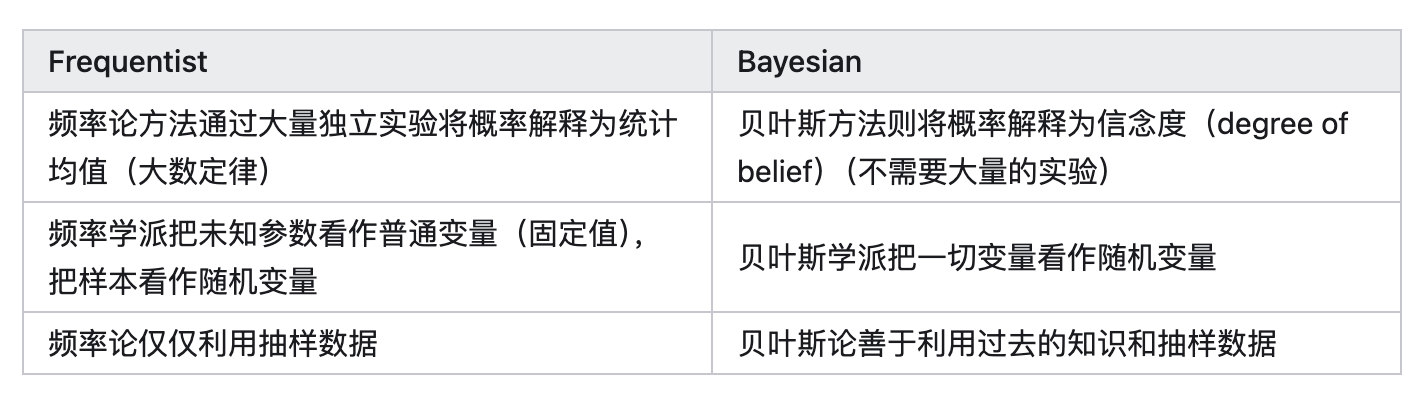
\includegraphics[scale=0.3]{figures/频率派和贝叶斯派.png}
    \caption{频率派和贝叶斯派}
\end{figure}



